\documentclass[doc,biblatex]{apa7}
\DeclareLanguageMapping{american}{american-apa}
\addbibresource{refs.bib}

\usepackage{amsmath}

\captionsetup[figure]{textfont=rm,font=small} % Override italic APA figure captions

\title{Simplicity and Informativeness in Semantic Category Systems}

\shorttitle{Simplicity and informativeness in semantic category systems}

\twoauthors{Jon W. Carr}{Kenny Smith, Jennifer Culbertson, Simon Kirby}

\twoaffiliations{Cognitive Neuroscience, International School for Advanced Studies, Trieste, Italy}{Centre for Language Evolution, University of Edinburgh, Edinburgh, UK}

\authornote{\textbf{Cite as:} Carr, J.\@ W., Smith, K., Culbertson, J., \& Kirby, S.\@ (2020). Simplicity and informativeness in semantic category systems. \textit{Cognition}, \textit{202}, Article 104289. https://doi.org/10.1016/j.cognition.2020.104289}

\abstract{Recent research has shown that semantic category systems, such as color and kinship terms, find an optimal balance between simplicity and informativeness. We argue that this situation arises through pressure for simplicity from learning and pressure for informativeness from communicative interaction, two distinct pressures that often (but not always) pull in opposite directions. Another account argues that learning might also act as a pressure for informativeness, that learners might be biased toward inferring informative systems. This results in two competing hypotheses about the human inductive bias. We formalize these competing hypotheses in a Bayesian iterated learning model in order to simulate what kinds of languages are expected to emerge under each. We then test this model experimentally to investigate whether learners' biases, isolated from any communicative task, are better characterized as favoring simplicity or informativeness. We find strong evidence to support the simplicity account. Furthermore, we show how the application of a simplicity principle in learning can give the impression of a bias for informativeness, even when no such bias is present. Our findings suggest that semantic categories are learned through domain-general principles, negating the need to posit a domain-specific mechanism.}

\keywords{category learning; induction; informativeness; iterated learning; language evolution; simplicity}

\begin{document}
\maketitle

%%%%%%%%%%%%%%%%%%%%%%%%%%%%%%%%%%%%%%%%%%%%%%%%%%%%%%%%%%%%%%%%%%%%%%%%%%%%%%%%%%%
\section{Introduction}
%%%%%%%%%%%%%%%%%%%%%%%%%%%%%%%%%%%%%%%%%%%%%%%%%%%%%%%%%%%%%%%%%%%%%%%%%%%%%%%%%%%

There is no singular, objective way of dividing the world into categories; different human populations align on different systems of categorization. In the domain of kinship, for example, different languages have different ways of grouping family members into labeled categories \parencite{Murdock:1970}. Cantonese, for example, makes a lexical distinction between all four grandparents---y\`{e}h (father's father), m\`{a}h (father's mother), g\={u}ng (mother's father), and p\`{o}h (mother's mother) \parencite{Cheung:1990}, while most varieties of English collapse the distinction between the maternal and paternal lineage. Despite this diversity in how languages classify meanings into categories, there is evidence to suggest that such category systems achieve a balance between simplicity (e.g., the number of categories that must be learned) and informativeness (e.g., the ability to express useful distinctions). Different languages find different solutions to this tradeoff (as in the comparison between Cantonese and English above), but they nevertheless offer a near optimal balance between the two properties.

There is a long tradition in the cognitive and language sciences of explaining such constraints on linguistic variation in terms of competing pressures for simplicity and informativeness \parencite[e.g.,][]{Gabelentz:1891,Zipf:1949,Martinet:1952}. In the context of semantic category systems, \textcite[p.~28]{Rosch:1978} argued that ``the task of category systems is to provide maximum information with the least cognitive effort,'' \textcite[p.~502]{Komatsu:1992} discussed ``the tension between informativeness and economy'' that exists in such systems, and \textcite[p.~132--133]{Gardenfors:2014} has said that concepts achieve ``a balance between the precision of the noun and the number of words that have to be remembered.'' More recently, informativeness has been explicitly linked to a notion of precise communication, as illustrated in this quotation from \textcite[][p.~111]{Kemp:2018}:

	\begin{quote}
	A highly informative communicative system would be very fine-grained, detailed, and explicit---and would as a result be complex, not simple. A very simple system, in contrast, would necessarily leave implicit or unspecified many aspects of the speaker's intended meaning---and would therefore not be very informative. A system supports efficient communication to the extent that it achieves an optimal trade-off between these two competing considerations.
	\end{quote}

\noindent This claim has been shown to hold in a variety of domains, including kinship terms \parencite{KempRegier:2012}, spatial relationships \parencite{Khetarpal:2013}, numeral systems \parencite{Xu:2014}, color terms \parencite{Regier:2015}, container names \parencite{Xu:2016}, and animal taxonomies \parencite{Zaslavsky:2019}. However, as \textcite[p.~989]{Levinson:2012} has pointed out, although this body of research demonstrates that natural languages are both simple and informative, and~that a tradeoff exists between these two properties, it does not specify the mechanisms that give rise to this state of affairs.

In direct response, \textcite{Carstensen:2015} offered a partial answer. The authors argue that language learners are biased toward inferring informative languages, thus providing a potential mechanism behind the presence of informativeness in semantic category systems. This was demonstrated in two experimental studies using the \textit{iterated learning} paradigm \parencite{Kirby:2008}. In this paradigm, an artificial language is transmitted from one participant to another. As the language is passed along a chain of learners, it gradually adapts to their cognitive biases, revealing what those biases are \parencite[for reviews, see][]{Kirby:2014,Tamariz:2017}. \textcite{Carstensen:2015} demonstrated that informative semantic categories can arise through this process, which therefore suggests that humans may have an inductive bias that favors informativeness. They showed this in two studies. In Study~1, the authors reanalyzed data from an iterated learning experiment with color terms by \textcite{Xu:2013}, and in Study~2, the authors conducted a novel iterated learning experiment using spatial relationship stimuli.

The idea that learning itself can give rise to informative systems is also supported by \textcite{Fedzechkina:2012}, albeit outside the domain of semantic categories. In their studies, adult learners restructure artificial languages in ways that appear to balance effort and ambiguity avoidance (i.e., informativeness). \textcite[][p.~17900]{Fedzechkina:2012} conclude that, ``...language learners are biased toward communicatively efficient linguistic systems and restructure the input language in a way that facilitates information transfer.''

However, these results are at odds with the prior research into iterated learning, which has repeatedly shown that learners have a bias for simplicity---not informativeness---and that iterated learning therefore gives rise to simple, degenerate, uninformative languages. Informative languages only emerge in the presence of a shared communicative task \parencite[e.g.,][]{Kirby:2015,Carr:2017,Saldana:2019,Motamedi:2019,Winters:2018,Raviv:2018} or an artificial analog of such a task \parencite{Kirby:2008,Beckner:2017}, neither of which was present in the two studies described by \textcite{Carstensen:2015}. One reason why learners might be biased toward simplicity is that, when learners are faced with understanding the world, the best strategy---given that they have no expectations about how the world is structured---is to apply Occam's razor; all things being equal, simpler hypotheses should be preferred over more complex ones \parencite{Solomonoff:1964a,Li:2008,Rissanen:1978}. This is a highly general principle, claimed to operate across cognitive domains \parencite{Chater:2003,Chater:2015,Culbertson:2016,Feldman:2016,Kemp:2012}, but its effect on linguistic and conceptual systems will be amplified by iterated learning, ultimately giving rise to simple languages.

This leaves us with a somewhat mixed picture. On the one hand, there is a long tradition of associating learning with simplicity, and a large body of iterated learning experiments show that learning ultimately has a simplifying effect on language structure. From this perspective, informativeness is usually argued to derive from another source, such as communicative interaction. But on the other hand, some recent studies argue that language learners may also be directly biased toward informative structures. This gives rise to two competing positions about the human inductive bias: Do human learners have an inductive bias toward simple languages or informative languages?

In an iterated learning model with Bayesian category learners, we show what kinds of languages are expected to emerge under a bias for simplicity and under a bias for informativeness. We then test the predictions of this model experimentally, and in an objective model comparison, we find that the human learning bias is better characterized by a preference for simplicity. Furthermore, we show how the application of a simplicity principle in learning can explain the apparently contradictory results described by \textcite{Carstensen:2015}: Under a bias for simplicity, iterated learning gives rise to simple category systems that happen to have one of the hallmark features of an informative category system---a compact structural organization. Thus, although it is true that informativeness, when defined a particular way, can emerge through iterated learning, this does \textit{not} imply that learners have a domain-specific bias for informativeness, since its emergence can also be explained by a domain-general bias for simplicity.

%%%%%%%%%%%%%%%%%%%%%%%%%%%%%%%%%%%%%%%%%%%%%%%%%%%%%%%%%%%%%%%%%%%%%%%%%%%%%%%%%%%
\section{Model}
%%%%%%%%%%%%%%%%%%%%%%%%%%%%%%%%%%%%%%%%%%%%%%%%%%%%%%%%%%%%%%%%%%%%%%%%%%%%%%%%%%%

In this section we describe an iterated learning model that simulates what happens when a language is passed down a chain of Bayesian learners. This reveals the kinds of languages that are expected to arise when pressure from learning---\textit{on its own}---is repeatedly applied. Furthermore, by manipulating the learning bias---represented by the prior function---we can test the two competing positions outlined in the Introduction. By formalizing the two positions in the form of a model, we make all assumptions explicit, and the predictions made by the model are directly testable.

\subsection{Method}

	\begin{figure}
	\makebox[\textwidth][c]{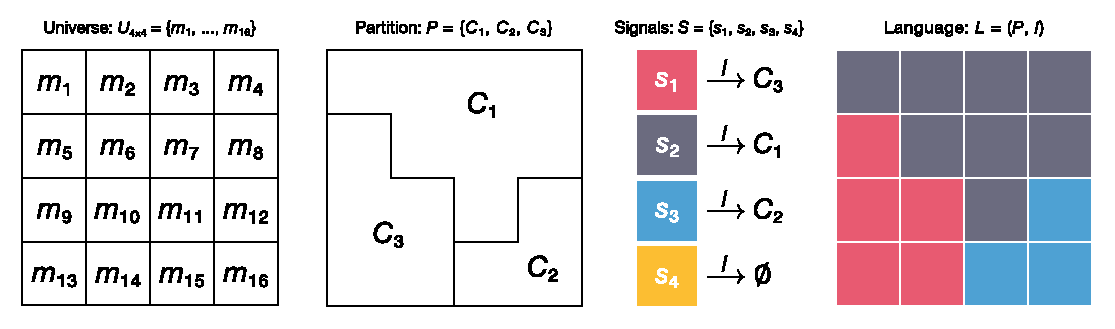
\includegraphics[]{fig01.eps}}
	\vspace*{2pt}
	\caption{From left to right: A universe is a two-dimensional metric space consisting of $M$ meanings; this space may be partitioned into $N$ mutually disjoint categories; agents are provided with a fixed set of $N_\mathrm{max}$ signals $S$, which are used to label the categories; a language defines how the space is partitioned into categories and how those categories are labeled. In this example, the language partitions a $4 \times 4$ space into three categories using three of the four available signals (each signal is represented by a color).}
	\label{fig01}
	\end{figure}

The basic model framework is illustrated in Fig.~\ref{fig01}. The universe consists of $M$ meanings $U = \{m_1, ..., m_M\}$, which we treat as a metric space~$(U, d)$, where $d$ is the distance function defined between meanings. Usually we will refer to this space simply as $U$, sometimes also denoting the dimensionality (e.g., $U_{4 \times 4}$ for a $4 \times 4$ space of $M = 16$ meanings). A partition~$P = \{C_1, ..., C_N\}$ divides $U$ into $N$ categories, such that $1 \leq N \leq N_\mathrm{max}$ where $N_\mathrm{max} \leq M$ defines some arbitrary limit on the number of categories. Each category $C$ is a set of meanings such that all categories are nonempty ($C_i \neq \emptyset$), no meaning exists outside a category ($\bigcup_{i=1}^{N} C_i = U$), and all categories are mutually disjoint ($C_i \cap C_j = \emptyset$ for~$i\neq j$). Each category is labeled by one signal from a fixed set of~$N_\mathrm{max}$ signals~$S = \{s_1, ..., s_{N_\mathrm{max}}\}$ according to a lexicon~$l : S \rightarrow P$ (if $N < N_\mathrm{max}$, the lexicon maps unused signals to $\emptyset$). A language is a partition and lexicon, $L = (P, l)$, and the goal of the learner is to infer what this language is---how the language partitions the universe into categories and how those categories are labeled. To do this, the Bayesian learner considers all possible language hypotheses---all possible ways the universe could be partitioned into labeled categories---and chooses the hypothesis that offers a good match with (a) the observed data, as defined by the likelihood, and (b) the learner's bias, as defined by the prior. We begin by describing the likelihood and then consider two possible priors.

\subsubsection{Likelihood}

The probability of an agent producing signal~$s \in S$ given that it possesses language~$L$ and needs to express meaning~$m$ is given by

	\begin{equation}
	p(s|L,m; \epsilon) =
		\begin{cases}
		  1 - \epsilon                        & \mathrm{if} ~ m \in l(s) \\
		  \frac{\epsilon}{N_\mathrm{max} - 1} & \mathrm{if} ~ m \notin l(s) ,
		\end{cases}
	\label{production}
	\end{equation}

\noindent where $l(s)$ is the category labeled by signal $s$ and noise is controlled by the free parameter~$\epsilon \in (0,1)$. If $\epsilon$ is small, there is a high probability that the agent will produce the correct signal for meaning $m$ and a low probability that it will produce one of the other $N_\mathrm{max} - 1$ signals at random. During learning, the data observed by an agent is a set of meaning--signal pairs $D = \{\langle m,s \rangle_1, \langle m,s \rangle_2, ...\}$, where meaning~$m$ is labeled by signal~$s$, a noisy indicator of $m$'s category membership. Consequently, the likelihood of observing dataset $D$ if language $L$ were true is the product of $p(s|L,m; \epsilon)$ for all observed meaning--signal pairs:

	\begin{equation}
	p(D|L; \epsilon) = \prod_{\langle m,s \rangle \in D} p(s|L,m; \epsilon).
	\label{likelihood}
	\end{equation}

\subsubsection{Simplicity Prior}

The simplicity prior endows agents with an inductive bias favoring simple languages; when the observed data is equally likely under two languages, an agent will prefer the language that is simpler following the principle of Occam's razor. The simplicity prior~$\pi_\mathrm{sim}$ is therefore inversely proportional to the complexity of the language:

	\begin{equation}
	\pi_\mathrm{sim}(L) \propto 2^{-\mathrm{complexity}(L)}.
	\label{prior_sim}
	\end{equation}

\noindent The complexity of a language is its minimum description length in bits. For our description method, we adopt Fass and Feldman's (\citeyear{Fass:2002}) rectangle code, which provides a set of rectangle ``symbols'' that may be used to describe an arbitrary region (i.e., a category's extension) in the universe. In $U_{4 \times 4}$, this method provides a total of 100 symbols, which are illustrated in Fig.~\ref{fig02}. A valid description of a category is a set of rectangle symbols that losslessly describe the category's extension, which we call a ``rectangularization'' of that category. For a given category~$C$, there are usually many possible rectangularizations (descriptions), the set of which is given by $\Re(C)$. A rectangularization~$R \in \Re(C)$ that minimizes description length is selected, and description lengths are then summed over all categories to obtain the overall complexity of a language:

	\begin{figure}
	\makebox[\textwidth][c]{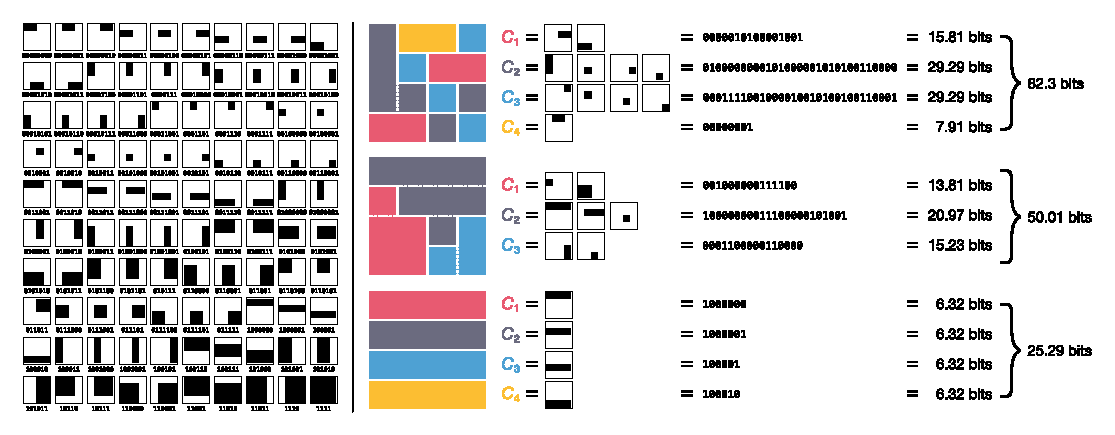
\includegraphics[]{fig02.eps}}
	\vspace*{2pt}
	\caption{Left: The 100-symbol rectangle code which is used to describe categories in a $4 \times 4$ universe; each symbol is shown with a binary codeword. Right: Three example languages and their complexity scores, as measured by the length of their shortest descriptions in the rectangle code. The first language, which was generated randomly, does not permit a short description and is therefore considered complex. The second language consists of three contiguous categories that permit shorter descriptions, so it is therefore considered less complex. The third language, which has a very short description, is the joint-simplest four-category language. The binary strings are for illustrative purposes and do not reflect the shortest possible descriptions that could be obtained under an ideal coding system.}
	\label{fig02}
	\end{figure}

	\begin{equation}
	\mathrm{complexity}(L) = \sum_{C \in L} \min_{R\in\Re(C)} \sum_{r \in R} -\log p(r),
	\label{complexity}
	\end{equation}

\noindent where $p(r)$ is the probability of a rectangle symbol occurring following the same assumptions outlined in \textcite[p.~38--39]{Fass:2002}. Illustrative examples are shown in Fig.~\ref{fig02}. For additional detail on these methods see \textcite[p.~91--97]{Carr:2019}, but note that we are essentially adopting a minimum description length approach \parencite{Rissanen:1978,Grunwald:2007}, in which the lossless compressibility of a hypothesis is used as an estimator of its simplicity.\footnote{This should not be confused with the fact that categories themselves are a form of lossy compression. In evaluating a category system (i.e., a candidate language hypothesis $L$), the simplicity-endowed agent is seeking the shortest lossless description of that system, but the system itself may be lossy (a single category encompasses multiple meanings) or lossless (every meaning belongs to its own distinct category) in terms of its representational or communicative precision (informativeness).}

This method encodes two main assumptions about the properties that make a semantic category system simple:

	\begin{enumerate}
		\item \textbf{Number of categories} The fewer categories a system has, the simpler that system is (i.e., complexity is lower).
		\item \textbf{Contiguity} The more contiguous categories are, the simpler the system is (i.e., complexity is lower).
	\end{enumerate}

\noindent Thus, under the simplicity bias, the learner will prefer systems that exhibit these two properties. Although the rectangle code does not fully capture the kinds of category systems tested in \textcite{Carstensen:2015}, we contend that it still offers a useful way to model a general preference for simplicity in semantic category systems. We return to this issue in the Discussion.

\subsubsection{Informativeness Prior}

To model an inductive bias for informativeness, we directly adopt the communicative cost framework used by \textcite{Carstensen:2015} and other studies from that literature \parencite[e.g.,][]{Regier:2015}. This prior endows agents with an inductive bias toward informative languages; when the observed data is equally likely under two languages, an agent will prefer the language that is more informative. The informativeness prior~$\pi_\mathrm{inf}$ is inversely proportional to the communicative cost of the language:

	\begin{equation}
	\pi_\mathrm{inf}(L) \propto 2^{-\mathrm{cost}(L)},
	\label{prior_inf}
	\end{equation}

\noindent and communicative cost is calculated according to:

	\begin{equation}
	\mathrm{cost}(L) = \sum_{C \in L} \sum_{m \in C} p(m) \cdot -\log p(m|C),
	\label{cost}
	\end{equation}

\noindent where $p(m)$ is the probability that a hypothetical speaker would wish to express meaning $m$ (assumed to be uniform; $p(m) = 1/|U|$) and $p(m|C)$ is the probability that a hypothetical listener would infer meaning $m$ on hearing the signal associated with category $C$:

	\begin{equation}
	p(m|C) \propto \sum_{m^\prime \in C} \exp -\gamma d(m,m^\prime)^2,
	\label{cost_listener}
	\end{equation}

	\begin{figure}
	\makebox[\textwidth][c]{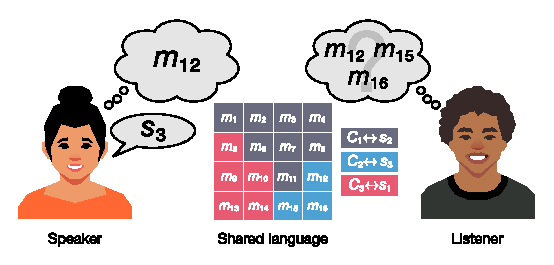
\includegraphics[]{fig03.eps}}
	\vspace*{2pt}
	\caption{A speaker wishes to communicate a target meaning (e.g., $m_{12}$) from a universe of meanings. She determines which category the target belongs to according to the language (e.g., $C_2$) and utters its associated signal (e.g., $s_3$). The listener maps this signal back to the category and must decide on a specific meaning to infer. In this example, the listener has three potential meanings to choose from, so the probability of a successful outcome is $1/3$. However, in many instances of the communicative cost model, including the one presented in this paper, the listener is more likely to infer prototypical (central) members of the category. An informative language, with low communicative cost, is structured in such a way as to minimize the potential loss of information that occurs during interaction.}
	\label{fig03}
	\end{figure}

\noindent where $\gamma > 0$ controls how quickly similarity decays with the distance between two meanings in $(U, d)$. In all work reported below, we set $\gamma = 1$ and $d(\cdot,\cdot)$ is the Euclidean metric. Eq.~\ref{cost_listener} models categories as Gaussians in which the most prototypical meaning (the meaning at the geometric center of the category with the greatest similarity to other category members) has the highest probability of being inferred by a hypothetical listener. A simple example of the communicative cost framework is illustrated in Fig.~\ref{fig03}. Importantly, note that no interaction is actually played~out between our agents; rather, the learner has a bias favoring languages that would hypothetically be more informative in expected communicative scenarios. For a more complete introduction to the communicative cost framework, consult the references above or \textcite[p.~38--44]{Carr:2019}.

This method encodes two main assumptions about the properties that make a semantic category system informative:

	\begin{enumerate}
		\item \textbf{Number of categories} The more categories a system has, the more informative that system is (i.e., communicative cost is lower).
		\item \textbf{Compactness} The more compact categories are, the more informative the system is (i.e., communicative cost is lower).
	\end{enumerate}

\noindent Thus, under the informativeness bias, the learner will prefer systems that exhibit these two properties. By ``compactness'' we mean the extent to which similar meanings belong to the same semantic category and dissimilar meanings belong to different semantic categories. This has also been described as ``well-formedness'' \parencite{Regier:2007}. Compact categories are considered informative in the communicative cost framework because it is assumed that listeners will tend to infer more prototypical meanings, so arranging categories compactly will tend to result in greater communicative precision.

\subsubsection{Posterior}

On observing data~$D$, the Bayesian learner samples a language hypothesis $L^\ast$ from the posterior distribution over the space of possible languages $\mathcal{L}$, which is given by Bayes' rule:

	\begin{equation}
	p(L|D; \pi,w,\epsilon) \propto p(D|L; \epsilon) \pi(L)^w.
	\label{posterior}
	\end{equation}

\noindent Here, $w$ is a free parameter determining the strength of the prior relative to the likelihood.\footnote{When $w=1$ the prior is left unchanged; when $w>1$, the prior is strengthened; when $0 < w < 1$ the prior is weakened; and when $w=0$ the prior is flattened to a uniform distribution.} In all work that follows, we set $N_\mathrm{max} = 4$ (an agent is limited to inferring at most four categories) and we assume an $8 \times 8$ universe, such that the number of language hypotheses is $|\mathcal{L}| = 4^{64}$. Since we cannot sample directly from a hypothesis space of this size, we use the Metropolis--Hastings algorithm, which is initialized with a random language~$L_0$. To select the language at the next step, $L_{i+1}$, we propose a candidate language~$L^\prime$ and then calculate the acceptance ratio~$\alpha$, given by the product of the posterior ratio and proposal ratio:

	\begin{equation}
	\alpha = \frac{p(L^\prime|D; \pi,w,\epsilon)}{p(L_i|D; \pi,w,\epsilon)} \cdot \frac{p(L_i|L^\prime)}{p(L^\prime|L_i)}.
	\label{acceptance_ratio}
	\end{equation}

\noindent To propose a new candidate, a rectangular region in $U_{8 \times 8}$ is chosen at random such that all meanings in that region belong to a single category according to $L_i$; these meanings are then transferred to one of the other three possible categories at random, forming the new candidate~$L^\prime$. This proposal function is asymmetric---$p(L^\prime|L_i) \neq p(L_i|L^\prime)$---which is accounted for by the proposal ratio in Eq.~\ref{acceptance_ratio}.\footnote{A simpler symmetric proposal function in which single meanings are moved between categories at each step is prone to getting stuck in local maxima, which limits the ability of the algorithm to freely explore the hypothesis space under either prior function. Note that this method is not biased toward introducing new rectangles because it only modifies the category membership of rectangular areas that already exist. See \textcite[p.~97--102]{Carr:2019} for additional detail on these methods.} Finally, the candidate language is accepted ($L_{i+1} = L^\prime$) if $\alpha \geq 1$ or with probability $\alpha$ if~$\alpha < 1$; otherwise the candidate is rejected and the previous state is retained ($L_{i+1} = L_i$). This process is repeated 5000 times, and the final state is taken to be a fair sample from the posterior ($L^\ast = L_{5000}$). Note that this sampling procedure is used by a single agent to induce its language and should not be confused with the iterated learning procedure described in the following section.

\subsubsection{Iterated Learning}

	\begin{figure}
	\makebox[\textwidth][c]{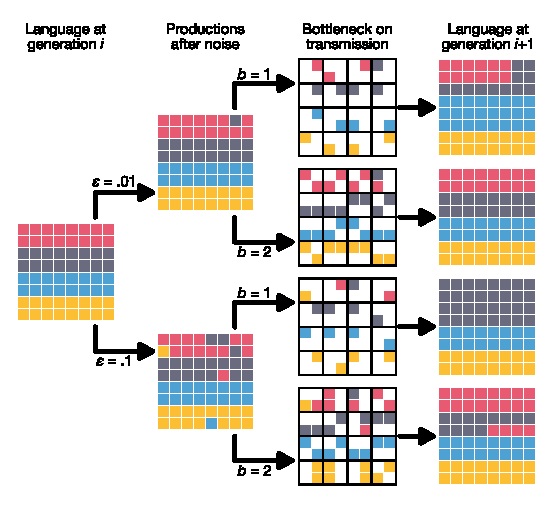
\includegraphics[]{fig04.eps}}
	\vspace*{2pt}
	\caption{Illustration of the transmission procedure over a single generation. The agent at generation~$i$ has a language, which it uses to produce signals with some probability of noise~$\epsilon$. These productions pass through the bottleneck on transmission: The universe is divided into 16 $2 \times 2$ segments, indicated here by the black grids, and $b$ meanings are selected from each segment. The agent at generation~$i+1$ only sees the signals associated with these meanings and, aided by the prior, must generalize to unseen meanings (empty white cells) forming a new language. The language is transmitted most faithfully when there is low noise (e.g., $\epsilon=.01$) and a wide bottleneck (e.g., $b=2$).}
	\label{fig04}
	\end{figure}

Agents are organized into chains such that the production output of one agent becomes the training input to the following agent in the chain, subject to noise on production and the bottleneck on transmission (a limit on how much information is transmitted from one generation to the next). An agent produces signals for each of the 64 meanings in $U_{8 \times 8}$ according to Eq.~\ref{production}, such that any given signal may be a production error with probability $\epsilon$. However, only some proportion of these 64 productions are actually observed by the next generation---only some pass through the bottleneck. This proportion is determined by the bottleneck parameter~$b$. To ensure that the agent observes meanings from all corners of the space, the productions were selected pseudorandomly: The $8 \times 8$ space is broken~up into 16 $2 \times 2$ segments and a fixed number of meanings $b \in \{1,2,3,4\}$ are randomly selected from each segment (see Fig.~\ref{fig04} for examples). Following other work in the iterated learning literature, the first agent in a chain learns from a randomly generated language. Finally, we also consider the exposure level~$\xi$ which controls how many exposures an agent gets to the productions that passed through the bottleneck (i.e., each meaning--signal pair that passes through the bottleneck is observed $\xi$ times).

\subsection{Results}

Our account of the results contrasts three prior biases: the simplicity prior with $w=1$, the informativeness prior with $w=1$, and a strong form of the informativeness prior with $w=500$. This strong form of the informativeness prior emphasizes the compactness property mentioned earlier; agents with this prior bias have a much stronger preference for compact categories. Results under these three biases are shown in Fig.~\ref{fig05} for the parameter settings $\epsilon=.01$, $b=2$, and $\xi=2$ (to explore the full set of model results under 48 parameter combinations, see the supplementary item or https://joncarr.net/p/shepard/). In all analyses in this paper, we consider four quantities of interest: the number of categories inferred, complexity (see Eq.~\ref{complexity}), communicative cost (see Eq.~\ref{cost}), and transmission error, which is measured as the variation of information \parencite{Meila:2007} between the language at generation $i$ and the language at generation $i-1$.\footnote{Variation of information (VI) is an information-theoretic distance metric between set partitions. Under this measure, an agent that infers exactly the same partition as the previous agent in the chain will have VI of 0~bits; maximum VI is $\log |U| = 6$~bits.}

	\begin{figure}
	\makebox[\textwidth][c]{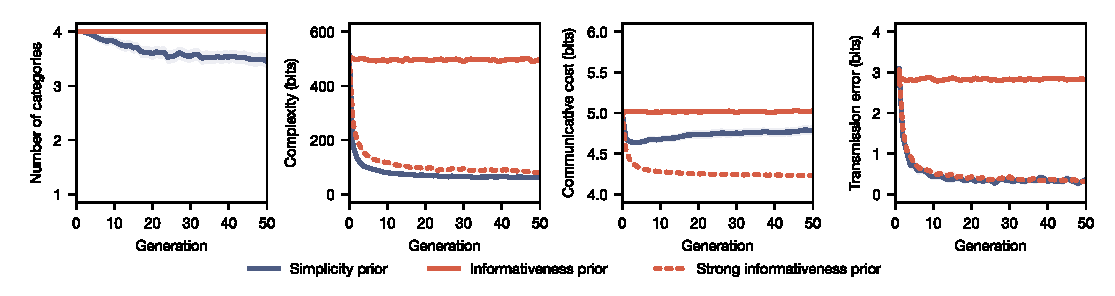
\includegraphics[]{fig05.eps}}
	\vspace*{2pt}
	\caption{Number of categories, complexity, communicative cost, and transmission error under the simplicity prior ($w=1$, solid blue lines), the informativeness prior ($w=1$, solid red lines), and a strong form of the informativeness prior ($w=500$, dashed red lines). Each line shows the mean of 100~chains over 50~generations, and the shaded areas show the 95\%~confidence intervals on the mean. In these runs of the model, agents saw half of the meanings ($b=2$) in two exposures ($\xi=2$) with a 1\% chance of noise ($\epsilon=.01$).}
	\label{fig05}
	\end{figure}

\subsubsection{Simplicity Prior}

The results under the simplicity prior are shown by the blue lines in Fig.~\ref{fig05} and a typical chain is depicted in Fig.~\ref{fig06}A. Over 50~generations, the languages become less complex, which is achieved in two ways: First, the categories take on simple, contiguous structures that may be described by a shorter description in the rectangle code; and second, categories are gradually lost over time, further simplifying the languages. This has an interesting effect on communicative cost, which initially drops---implying more informative languages---but then begins to rise again. This is because the contiguous categories that initially emerge are generally quite compact, and since communicative cost is sensitive to compactness, it initially decreases. But this effect is then gradually eroded by the loss of categories. Furthermore, the category structures that arise under the simplicity prior tend to mark distinctions on just one of the two dimensions; in the example in Fig.~\ref{fig06}A, the language ends up marking a three-way distinction on the \textit{x}-axis. This overall process of simplification results in more learnable languages, as indicated by decreasing transmission error over time. Within around 10 generations, the languages have simplified into configurations that are reliably transmitted from one generation to the next, despite the fact that agents only receive input data for half ($b=2$) of the meanings.

	\begin{figure}
	\makebox[\textwidth][c]{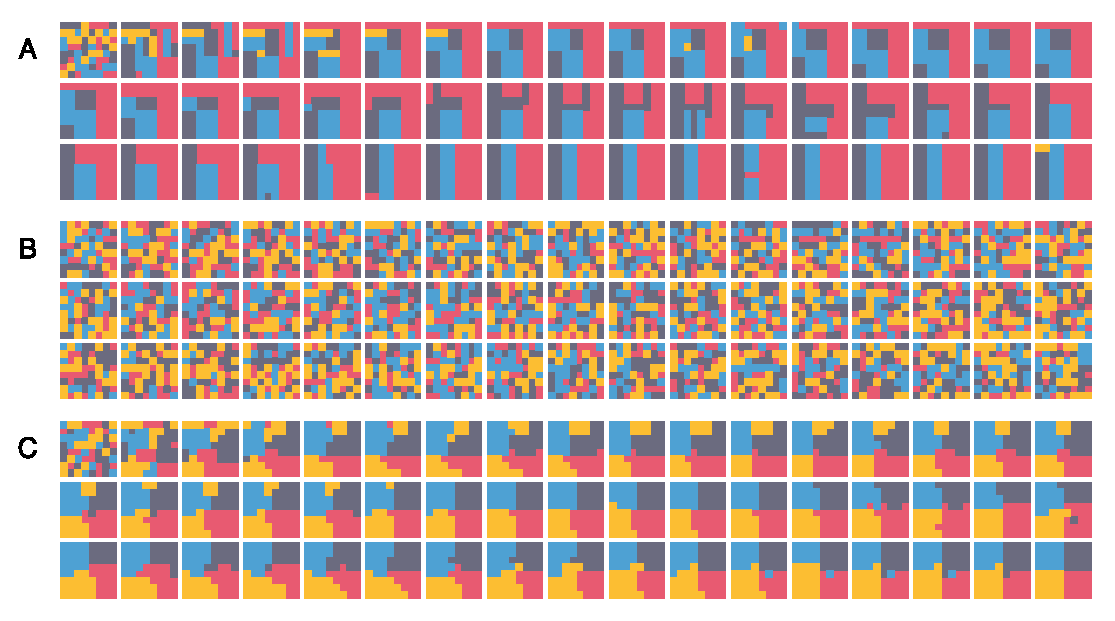
\includegraphics[]{fig06.eps}}
	\vspace*{2pt}
	\caption{An example chain for each of the three prior biases: (A) the simplicity prior, (B) the informativeness prior, and (C) the strong informativeness prior. Each chain starts with a randomly generated language (top-left) and is followed by 50 generations of iterated learning (from top-left to bottom-right).}
	\label{fig06}
	\end{figure}

\subsubsection{Informativeness Prior}

The results under the unweighted informativeness prior ($w=1$) are shown by the solid red lines in Fig.~\ref{fig05} (see Fig.~\ref{fig06}B for a typical example). The bias for informativeness causes the agents to maintain all four categories, and there is no effect on complexity, communicative cost, or transmission error. This is because the prior is very flat with respect to compactness and mostly encodes a preference for more categories, which cannot be obtained because of the $N_\mathrm{max}=4$ limit that we have imposed. If we were to remove this limit, the number of categories would eventually rise to 64 (every meaning forms its own category), communicative cost would decrease to its minimum value of 0~bits, and complexity would increase to its maximum value of around 715~bits.

\subsubsection{Strong Informativeness Prior}

The dashed red lines in Fig.~\ref{fig05} show results under the strong informativeness prior ($w=500$; see Fig.~\ref{fig06}C for an example). When the informativeness prior is strengthened in this way, all four categories continue to be maintained, but communicative cost also experiences a sustained decrease because the stronger prior favors categories that are maximally compact. This pressure for compactness drives chains toward one special partition of the universe: the partition into quadrants, as seen in the final generation in Fig.~\ref{fig06}C. This quadrant partition is the optimal packing of the space into four equally-sized categories. Under this prior, the learner has a strong expectation that categories will be arranged as compactly as possible and is therefore biased toward inferring such compact structure.

\subsubsection{Convergence to the Prior}

The extent to which chains converge to the prior bias---be it for simplicity or informativeness---is essentially controlled by intergenerational information~loss, which \textcite{Spike:2017} identify as an essential requirement for the emergence of structured languages. The greater the information loss, the faster the convergence to the prior. In other words, the less data an agent has to rely on, or the more unreliable that data is, the more the agent must lean on its prior bias to reconstruct the language. This is illustrated in Fig.~\ref{fig07}; there is greater convergence to the prior bias when the bottleneck is tighter, there are fewer exposures, or the level of noise is greater.

	\begin{figure}
	\makebox[\textwidth][c]{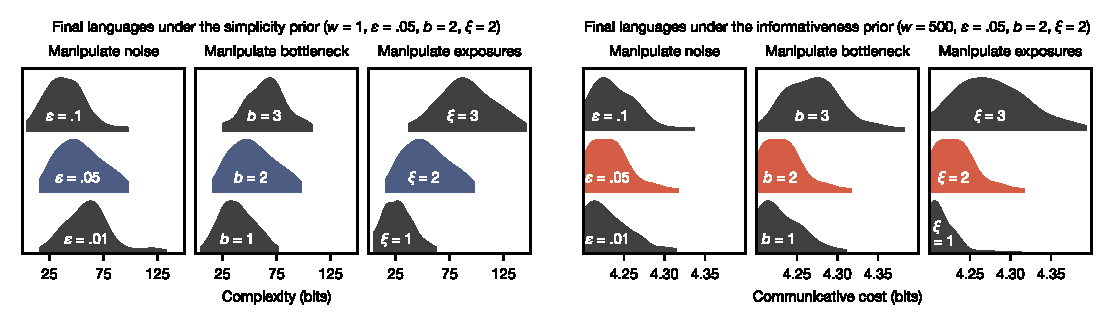
\includegraphics[]{fig07.eps}}
	\vspace*{2pt}
	\caption{Each density plot shows how complexity (left) or communicative cost (right) is distributed in the final-generation languages across 100 chains. The distributions in blue are identical and provide baseline results under the simplicity bias. Likewise, the distributions in red are identical and provide baseline results under the strong informativeness bias. The distributions in black show what happens when one parameter is manipulated, while holding all other parameters constant. Chains show greater convergence toward the prior bias when there is more noise, a tighter bottleneck, or fewer exposures. For example, decreasing the number of exposures from two to one gives rise to simpler languages under the simplicity bias and more informative languages under the informativeness bias.}
	\label{fig07}
	\end{figure}

\subsection{Summary}

We have put forward a model of a Bayesian category learner, and we have considered two prior functions: one for simplicity and one for informativeness. These two priors represent two extreme theoretical positions that one may take in regard to the learning of semantic categories, as outlined in the Introduction. In addition, we consider what happens when the informativeness prior is strengthened such that its compactness component is magnified. The results show that, when the number of categories is limited to four (i.e., $N_\mathrm{max} = 4$), as is the case in \textcite[][Study~2]{Carstensen:2015}, communicative cost only decreases over time, as the authors observed, in one of two situations:

	\begin{enumerate}
		\item Communicative cost decreases with generation if learners have a simplicity bias, but this decrease is \textit{not} sustained in the long run.
		\item Communicative cost decreases with generation if learners have an informativeness bias, but only if the compactness component of the bias is sufficiently strong.
	\end{enumerate}

\noindent If the simplicity prior offers a better model of the human inductive bias, we would expect to find that iterated learning results in contiguous category structures that make distinctions on principally one dimension and perhaps also a loss of some categorical distinctions altogether. If the informativeness prior offers a better model, we would expect to find that iterated learning maintains the number of categorical distinctions and---if the compactness component of the bias is sufficiently strong---leads to maximally compact category structures. We now test these predictions in an experimental analog of our model.

%%%%%%%%%%%%%%%%%%%%%%%%%%%%%%%%%%%%%%%%%%%%%%%%%%%%%%%%%%%%%%%%%%%%%%%%%%%%%%%%%%%
\section{Experiment}
%%%%%%%%%%%%%%%%%%%%%%%%%%%%%%%%%%%%%%%%%%%%%%%%%%%%%%%%%%%%%%%%%%%%%%%%%%%%%%%%%%%

The experiment is largely identical to the model except that the Bayesian agents are replaced with human learners. The prior bias ($\pi$), its weight ($w$), and the noise level ($\epsilon$) are considered unknown parameters of the human learner; in a later section we estimate these parameters from the experimental data. The bottleneck parameter ($b$) and exposure level ($\xi$) are considered properties of the environment and are therefore fixed by the experiment. By maintaining close contact with the model, the experiment allows us to directly test the two competing positions formalized in the model and objectively determine which hypothesis about the human inductive bias is more likely to be true.

\subsection{Method}

The experiment is a simple category learning task comprised of a training phase (approximately 15~min) and a test phase (approximately 5~min). Participants are first taught labels for half of the stimuli and are then asked to produce labels for all stimuli. Thus, like the Bayesian agents, the human learners must generalize from their limited input in order to form a hypothesis about the full language. Unbeknown to the participants, the output produced during the test phase is passed~on to a new participant, whose production output is in turn passed~on to another new participant, and so forth.

\subsubsection{Participants}

224 participants were recruited through the Figure~Eight platform (https://www.figure-eight.com).\footnote{A total of 273 participants began the experiment; one was excluded for repeatedly clicking the same response button and a further 48 terminated the experiment prior to completing it.} Participants were paid \$3.00 plus up~to~\$1.92 in bonuses based on the accuracy of their learning (as detailed below). Ethical approval was granted by the School of Philosophy, Psychology and Language Sciences at the University of Edinburgh. All participants provided informed consent.

\subsubsection{Stimuli}

	\begin{figure}
	\makebox[\textwidth][c]{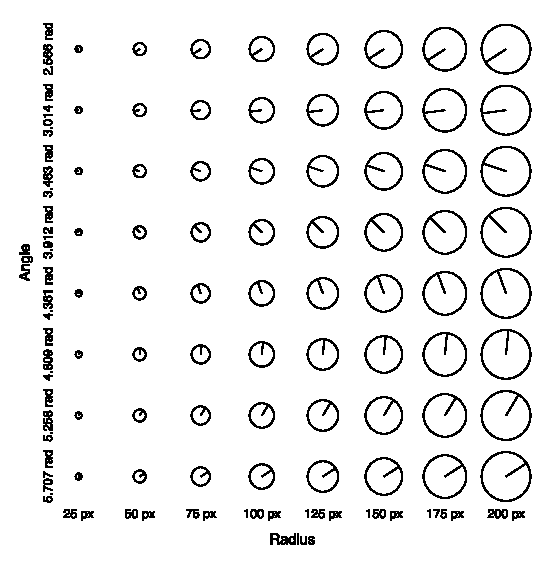
\includegraphics[]{fig08.eps}}
	\vspace*{2pt}
	\caption{The stimulus space varies continuously on two dimensions: the radius of the circle (\textit{x}-axis) and the angle at which the line is oriented (\textit{y}-axis). Each dimension is quantized into eight discrete values, yielding 64 stimuli.}
	\label{fig08}
	\end{figure}

We adopted the so-called ``Shepard circles'' \parencite{Shepard:1964} as our stimulus space (see Fig.~\ref{fig08}), which vary continuously in angle and size. The space was quantized onto an $8 \times 8$ grid, yielding 64 discrete stimuli. The radii vary between 25 pixels and 200 pixels and the angles vary over 180$^{\circ}$. The stimuli closely replicate the Shepard circles used by \textcite[][Fig.~1, p.~787]{Canini:2014}, who showed in a multidimensional scaling analysis that participants' dissimilarity perceptions of these stimuli are closely correlated with the Euclidean distance in the $8 \times 8$ grid. This makes the stimuli well justified analogs of the abstract meanings used in the model and allows us to assume that the Euclidean distance in the $8 \times 8$ grid is an acceptable approximation of perceived dissimilarity.

The category labels were three-letter nonwords (see Table~\ref{category_labels}). To create the labels, we generated all CVC strings, such that the first consonant letter was not the same as the final one, and then removed valid English words (e.g., \textit{pin}). For each of the remaining candidate labels, we attempted to translate the word into English from each of the 63 languages that use the Latin script in Google Translate. If Google was unable to offer a translation, we assumed that the label was not a real word in that language. We then selected 16 unique labels that were meaningless in as many languages as possible, such that they could be arranged into four sets of four labels in which any given set used no letter more than once. Each participant was assigned one set of labels selected at random, and the mapping between labels and categories was randomized for every participant. This procedure was designed to mitigate possible interference from native language and to reduce the possibility of iconic meaning--signal correspondences emerging, potentially making some mappings easier to learn than others \parencite[see e.g.,][]{Nygaard:2009,Nielsen:2012}.

	\begin{table}
	\begin{center}
	\begin{threeparttable}
	\caption{Category Labels}
	\begin{tabular}{lcccc}
	\hline
	\bfseries Set & \multicolumn{4}{c}{\bfseries Labels} \\ \hline
	1 & \textit{pov} & \textit{reb} & \textit{wud} & \textit{zix} \\
	2 & \textit{gex} & \textit{juf} & \textit{vib} & \textit{wop} \\
	3 & \textit{buv} & \textit{jef} & \textit{pid} & \textit{zox} \\
	4 & \textit{fod} & \textit{jes} & \textit{wix} & \textit{zuv} \\ \hline
	\end{tabular}
	\label{category_labels}
	\end{threeparttable}
	\end{center}
	\end{table}

\subsubsection{Training Procedure}

In the training phase, participants were trained on half of the 64 stimuli (i.e., $b=2$). These 32 stimuli were selected pseudorandomly through the same bottlenecking procedure used in the model (see Fig.~\ref{fig04}), which ensures that participants see a representative sample of meanings from all parts of the space. Training on the 32 items was repeated four times (i.e., in four blocks; $\xi=4$) because initial piloting indicated that participants would need at least four exposures to perform well above chance.

In each training block, the participant was exposed to each of the training items in random order. In a single trial (see Fig.~\ref{fig09}), the stimulus was presented first, and after a one-second delay, the sentence ``This is a \textbf{zix}'' appeared containing the relevant category label; this sentence remained on screen for 3~s, at which point it was replaced by the question ``What is it called?'' along with four buttons showing the four possible labels (the order of the response buttons was randomized on every trial). If the participant clicked the correct button, the button turned green; if incorrect, the button turned red and the button for the correct label turned green. After every fourth training trial (i.e., eight times per block, 32 times in total), a ``mini-test'' was inserted. In a mini-test trial, the participant is shown a previously seen stimulus and asked to supply a label for it. Feedback was then provided as in regular training trials, and the participant was awarded \$0.02 for every correct mini-test response. The purpose of the mini-tests and bonusing scheme was to make participants highly incentivized to learn the language as well as possible through active engagement with the training process.

	\begin{figure}
	\makebox[\textwidth][c]{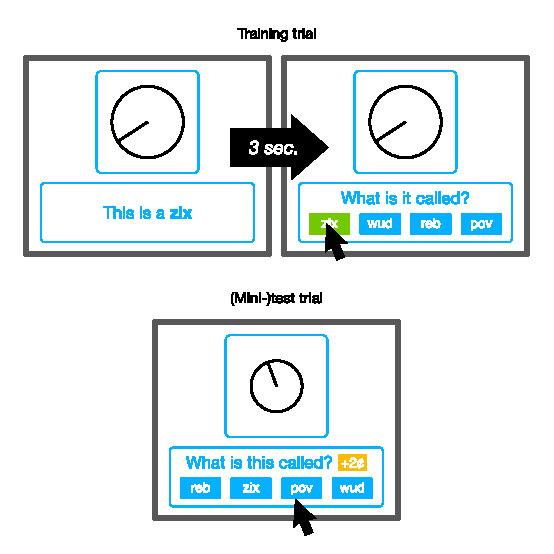
\includegraphics[]{fig09.eps}}
	\vspace*{2pt}
	\caption{Illustration of training and test trials (not to scale). In training trials, the participant is shown a stimulus and its category label, and after 3~s they are asked to click the correct label. In mini-test and test trials, the participant is shown a stimulus and asked to select a category label. Feedback is only provided in the case of mini-test trials.}
	\label{fig09}
	\end{figure}

\subsubsection{Test Procedure}

In the test phase, participants were asked to label all 64 stimuli. On each test trial, a stimulus was presented alongside the question ``What is this called?'' (see Fig.~\ref{fig09}). After a 1~s delay, the set of four labels appeared below in random order. It was made clear to the participant that they would be awarded \$0.02 for every correct response; however, no feedback was given during the test phase in order to elicit responses based on the hypothesis fixed during training.

\subsubsection{Transmission Procedure}

As in the model, the initial participant in a chain was given a randomly generated language to learn. The language they produced during the test phase was then transmitted to a new participant, subject to the same bottlenecking procedure as the model. Participants were assigned to one of~12 chains at random, and chains were run for a minimum of 10~generations. After the 10th generation, we allowed the chains to continue running until they eventually converged on a particular categorization system. Chains were deemed to have converged when two consecutive participants inferred exactly the same language, suggesting that that language was especially easy to learn---an attractor in the space of possible languages.

\subsection{Results}

	\begin{figure}
	\makebox[\textwidth][c]{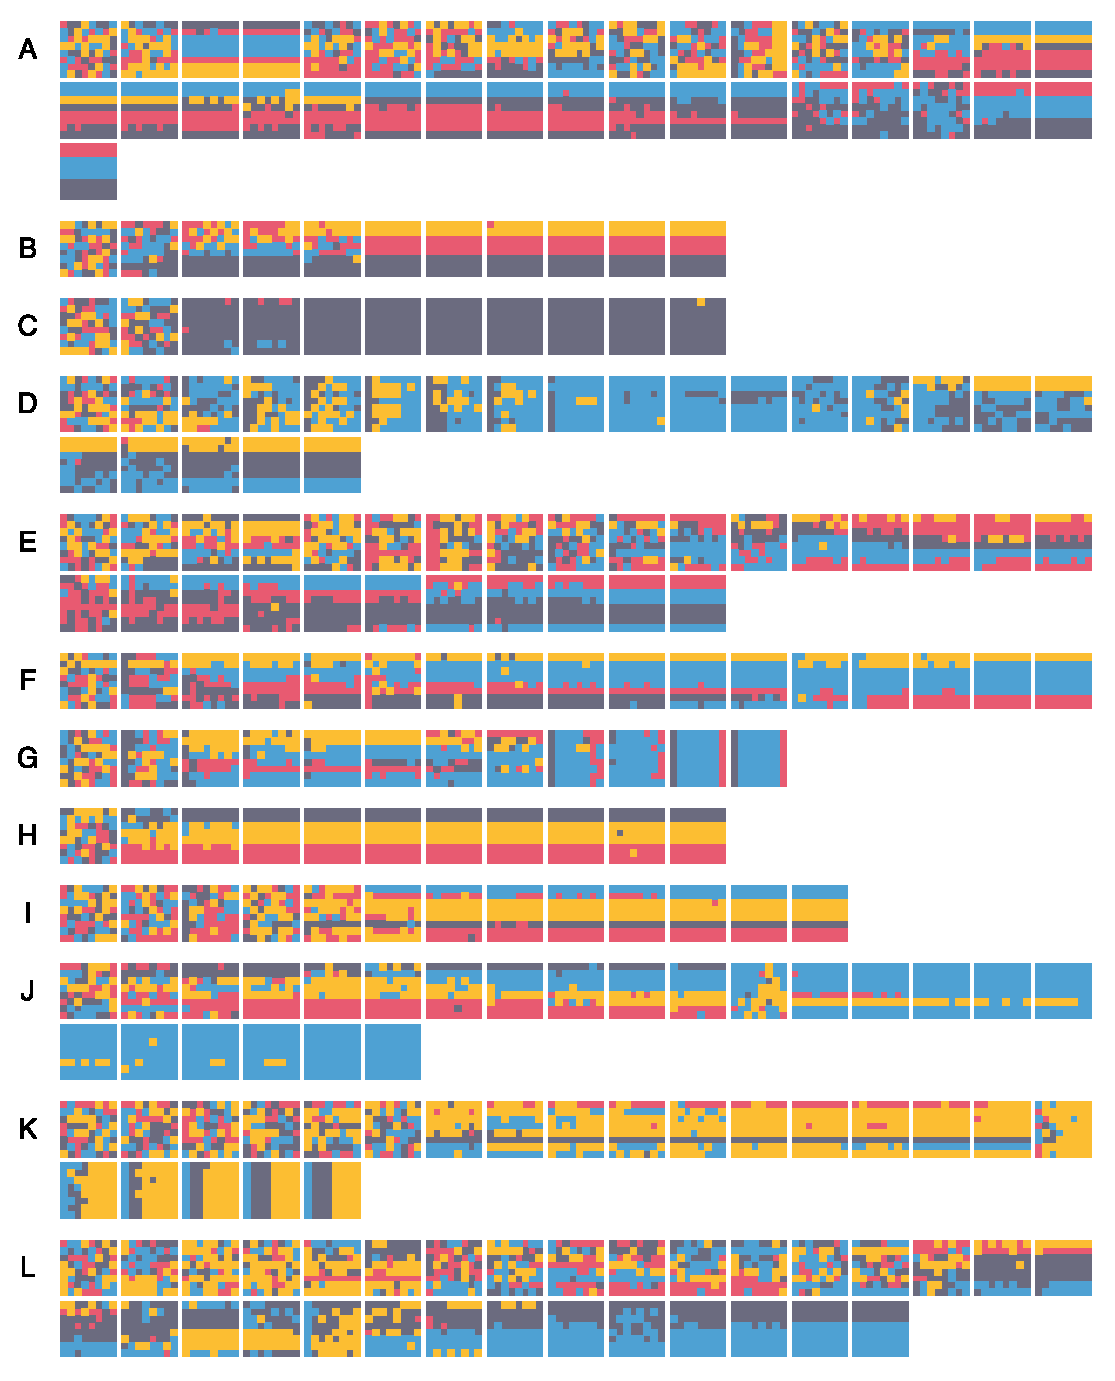
\includegraphics[scale=0.9]{fig10.eps}}
	\vspace*{2pt}
	\caption{Evolution of all~12 chains from the experiment (labeled A--L). Each chain starts with a randomly generated language and is followed by the language produced by each subsequent participant (from left to right; some chains are split across multiple rows). Chains were run for a minimum of 10 generations and then until two consecutive participants produced identical languages. Refer to Fig.~\ref{fig08} for the stimuli.}
	\label{fig10}
	\end{figure}

Fig.~\ref{fig10} depicts the evolution of all~12 chains (labeled A--L) through~to convergence, and the converged-on languages are summarized in Fig.~\ref{fig11}. In two cases, the languages collapsed to a single category; in one case, a two-category system emerged; and in eight cases, a three-category system emerged. Only in one case did the language retain all four categories (Chain~I). Fig.~\ref{fig11} also highlights the category structures that emerged. In eight cases (dashed black box), a system of contiguous categories emerged marking distinctions on the angle dimension, while in two cases (dashed gray box), a system of contiguous categories emerged marking distinctions on the size dimension. These findings speak directly to the predictions made by the simplicity prior in the model: We observe a loss of category distinctions and the emergence of simple, contiguous category structures that make distinctions on principally one dimension. The preference for marking the angle dimension perhaps reflects some form of saliency bias (e.g., angle jumps out as being more unusual and therefore more important to mark) or some form of perceptual bias (e.g., gradations in angle are easier to perceive).

	\begin{figure}
	\makebox[\textwidth][c]{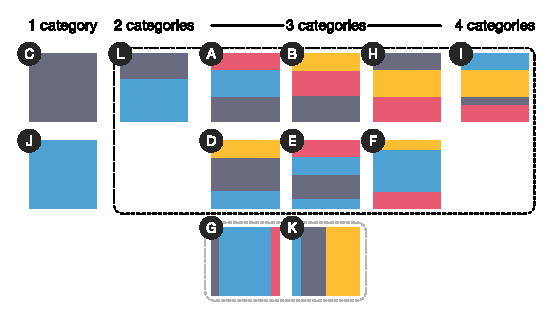
\includegraphics[]{fig11.eps}}
	\vspace*{2pt}
	\caption{The languages that were converged on across all~12 chains (labeled A--L) grouped by number of categories. Eight of the emergent languages mark distinctions in angle (dashed black box) and two of the languages mark distinctions in size (dashed gray box). Refer to Fig.~\ref{fig08} for the stimuli.}
	\label{fig11}
	\end{figure}

	\begin{figure}
	\makebox[\textwidth][c]{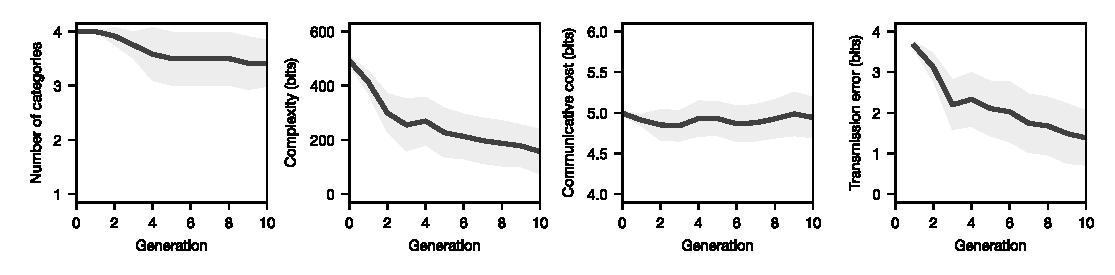
\includegraphics[]{fig12.eps}}
	\vspace*{2pt}
	\caption{Experimental results for the first 10 generations. Over time the languages become simpler and begin to use fewer categories. As a result of this simplification, they become more reliably transmitted from one generation to the next. Communicative cost remains static implying that the languages are not becoming more informative.}
	\label{fig12}
	\end{figure}

Fig.~\ref{fig12} shows the results under the same four quantitative measures computed for the model. Results are shown only for the first 10~generations, for which we have data from all~12 chains. A linear mixed-effects regression analysis was used to test for an effect of generation on each of the four measures with chain as a random effect and by-chain random slopes for the effect of generation, following the procedure recommended by \textcite{Winter:2016} and using the R package lme4 \parencite{Bates:2015}. \textit{P}-values were obtained by likelihood ratio tests of the full model against a null model without the effect in question. As predicted by our model simplicity bias, number of categories ($\beta = -0.06 \pm 0.03$, $\chi^2 = 5.19$, $p = .023$), transmission error ($\beta = -0.22 \pm 0.05$, $\chi^2 = 13.22$, $p < .001$), and complexity ($\beta = -22.59 \pm 6.12$, $\chi^2 = 9.67$, $p = .002$) all decreased with generation. Over time, the languages become structurally simpler and use fewer categories, and are, as a result, more faithfully transmitted. Contrary to \textcite{Carstensen:2015}, we did not find a decrease in communicative cost over generations ($\beta = 0.009 \pm 0.01$, $\chi^2 = 0.46$, $p = .499$), implying that the languages are \textit{not} becoming more informative.

\subsection{Model Fit}

To objectively determine which of the two prior functions offers a better fit to our experimental dataset $\mathcal{D}$, we calculate the likelihood that a participant would produce certain output data $D_\mathrm{out}$ given certain input data $D_\mathrm{in}$, and then take the product of this value over all\footnote{The model fit was performed on data from 168 of the 224 participants (75\%). We excluded participants whose transmission error was greater than 3~bits, since including them led to very high estimates of noise and a poor fit under either of the priors. In other words, for the purpose of the model fit, we retained only those participants whose productions were not wildly divergent from their input data.} participants:

	\begin{equation}
	p(\mathcal{D} | \pi,w,\epsilon) = \prod_{\langle D_\mathrm{in}, D_\mathrm{out} \rangle \in \mathcal{D}} p(D_\mathrm{out}|L^\ast; \epsilon),
	\label{modelfit_likelihood}
	\end{equation}

	\begin{figure}
	\makebox[\textwidth][c]{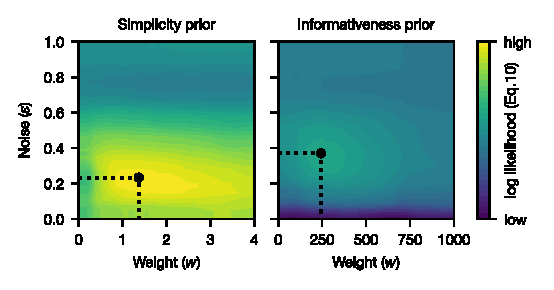
\includegraphics[]{fig13.eps}}
	\vspace*{2pt}
	\caption{Model fit results for the simplicity prior (left) and informativeness prior (right). Each plot shows how the weight and noise parameters affect the likelihood of observing the experimental dataset. Yellow areas indicate settings of $w$ and $\epsilon$ that offer a good fit to the experimental data. The black dots show the maximum likelihood estimates, the parameter values found to maximize Eq.~\ref{modelfit_likelihood}.}
	\label{fig13}
	\end{figure}

\noindent where $p(D_\mathrm{out}|L^\ast; \epsilon)$ is given by Eq.~\ref{likelihood} and $L^\ast$ is sampled from $p(L|D_\mathrm{in}; \pi,w,\epsilon)$ following Eq.~\ref{posterior}. In other words, for each participant (for each $\langle D_\mathrm{in}, D_\mathrm{out} \rangle$ pair in the dataset), we simulate what language an agent would infer given the participant's $D_\mathrm{in}$ and then calculate the likelihood of that agent producing the participant's $D_\mathrm{out}$ given that language. Then, for each of the prior functions, $\pi_\mathrm{sim}$ and $\pi_\mathrm{inf}$, we estimate $\hat{w}, \hat{\epsilon} = \operatornamewithlimits{arg\,max}_{w,\epsilon} p(\mathcal{D} | \pi,w,\epsilon)$, the parameter values that maximize Eq.~\ref{modelfit_likelihood}. Maximum likelihood estimates were obtained using the Python package scikit-optimize \parencite{scikitOptimize}. $\epsilon$ was bounded in $(0,1)$. $w$ was bounded in $[0,4]$ for the simplicity prior and $[0,1000]$ for the informativeness prior. The upper bounds were selected based on initial experimentation, which indicated that the likelihood would drop off beyond these values.

The results of the model fit are shown in Fig.~\ref{fig13}. For the simplicity prior, the maximum likelihood estimates are $\hat{w}_\mathrm{sim} \approx 1.37$ and $\hat{\epsilon}_\mathrm{sim} \approx .23$, yielding a log likelihood of $-11323.09$. For the informativeness prior, the maximum likelihood estimates are $\hat{w}_\mathrm{inf} \approx 243.3$ and $\hat{\epsilon}_\mathrm{inf} \approx .37$, yielding a log likelihood of $-17283.35$. These results tell us that, overall, the best fit to the experimental data is given by a slightly strengthened simplicity prior with a noise level of around 23\%. For the informativeness prior, the best fit is obtained by strengthening it substantially and assuming a noise level of around 37\%. The likelihood ratio is $2^{5960}$, offering overwhelming evidence that the simplicity prior gives a better fit to the experimental data than the informativeness prior.

Rerunning the iterated learning model with the parameter settings $b=2$, $\xi=4$ (as fixed by the experiment), $w=\hat{w}$, and $\epsilon=\hat{\epsilon}$ (as estimated from the experimental data), we obtain the results shown in Fig.~\ref{fig14}. The experimental results are shown for comparison: Results for the first 10 generations are reproduced from Fig.~\ref{fig12} and results for the subsequent 40~generations (dashed line) are estimated based on the assumption that once a chain fully converges it will experience no further change.\footnote{In~fact, we would expect to see a further reduction in complexity in the experimental results were it financially practical to run all~12 chains for 50~generations. Nevertheless, the assumption that chains are unlikely to change once they converge is not entirely unwarranted: As can be seen in Chains B, C, and H (see Fig.~\ref{fig10}), once a chain fully converges, the category structure tends to be reliably conserved over subsequent generations.} These plots confirm that the simplicity prior yields a general pattern of results that correspond closely to the experimental evidence.

	\begin{figure}
	\makebox[\textwidth][c]{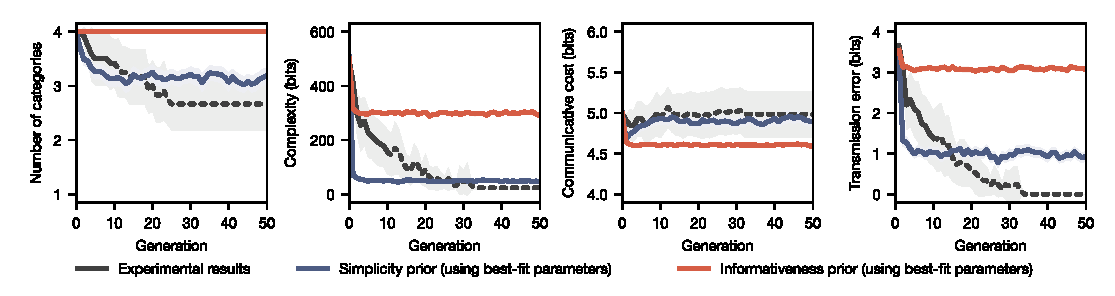
\includegraphics[]{fig14.eps}}
	\vspace*{2pt}
	\caption{Model results under the simplicity prior (blue) and informativeness prior (red) using parameter values estimated from the experimental data. For comparison, the experimental results are shown in black; the dashed part of the line beyond generation 10 is based on the assumption that a chain will not change once it converges (see main text). Shaded areas show the 95\% confidence intervals on the mean.}
	\label{fig14}
	\end{figure}

However, Fig.~\ref{fig14} also reveals two discrepancies between the experiment and the modeled simplicity bias: First, the simplicity prior results in a rapid, early decrease in complexity (unlike the experiment where complexity decreases more gradually), and second, it results in high transmission error later in the chains (unlike the experiment where transmission error tends toward 0 as the languages become very easy to learn). These discrepancies are a result of our simplistic model of noise, which is constant over generations and does not capture the fact that some types of error occur more often than others. In reality, noise appears to be some function of how complex a language is or how much confidence a participant has in their hypothesis, and participants are also more likely to make certain errors over others (e.g., greater confusion at category boundaries). These aspects of the real dynamics are not captured by our model and could be the subject of future work.

\subsection{Summary}

Our experiment shows that, when there is only a pressure from learning, languages evolve to become as simple as possible. Simplicity is achieved by reducing the number of categories and transitioning toward contiguous, one-dimensional category structures. These results are closely aligned with our model simplicity bias; indeed, fitting the model to the experimental data shows that the results are much better predicted by a preference for simplicity. Furthermore, unlike \textcite{Carstensen:2015}, the languages did not become more informative over generational time. The increase in the contiguity of the categories (spurred~on by the preference for simplicity) should in~fact make the languages more informative; but this effect was simultaneously countered by the loss of categorical distinctions, which makes the languages less informative, resulting in a flat line for communicative cost (see Fig.~\ref{fig12}).

%%%%%%%%%%%%%%%%%%%%%%%%%%%%%%%%%%%%%%%%%%%%%%%%%%%%%%%%%%%%%%%%%%%%%%%%%%%%%%%%%%%
\section{Discussion}
%%%%%%%%%%%%%%%%%%%%%%%%%%%%%%%%%%%%%%%%%%%%%%%%%%%%%%%%%%%%%%%%%%%%%%%%%%%%%%%%%%%

In a variety of typological studies, Regier and colleagues have shown that communication systems strike a balance between simplicity and informativeness \parencite[e.g.,][]{KempRegier:2012,Khetarpal:2013,Xu:2014,Regier:2015,Xu:2016,Zaslavsky:2019}. However, until recently, this body of work had avoided positing causal explanations behind this observation \parencite[p.~989]{Levinson:2012}. In direct response to that criticism, \textcite{Carstensen:2015} conducted an iterated learning experiment purporting to show that the learning of semantic category systems can contribute to increased informativeness in such systems. However, this account runs contrary to the iterated learning literature, which has generally shown that learning alone favors simple communication systems, with informativeness only emerging in the presence of a shared communicative task \parencite[e.g.,][]{Kirby:2015}. Such a task was not present in either of the studies described by \textcite{Carstensen:2015}, so how are we to explain their finding that informativeness can increase merely as a consequence of iterated learning?

The answer suggested by \textcite{Carstensen:2015} is that learners have an a-priori expectation that languages ought to be informative and that they are therefore biased toward inferring more informative systems over less informative systems. If, for example, the evidence presented to a learner was equally compatible with an informative system and an uninformative system, this biased learner would infer the informative one. This bias could be quite strong or quite weak, but either way, when the learning process is repeatedly applied to a language (iterated learning), it is amplified, gradually nudging the language in the direction of greater informativeness.

Our alternative answer is perhaps more mundane. As noted earlier, the authors' measure of informativeness---communicative cost---is sensitive to how ``structured'' the categories are. Specifically, it is sensitive to how compactly the categories are arranged; category systems in which similar meanings tend to be classified into the same category are considered more informative than those that do not have such structure. Putting aside the issue of whether this is a desirable feature of a measure of informativeness, the problem that arises from this definition is that such structure could also be described as simple (we return to this point shortly). Thus, when we observe the emergence of structured categories, it is not immediately clear whether the languages are adapting to become more informative or to become more simple. In short, we argue that \textcite{Carstensen:2015} have attributed the emergence of category structure to a pressure for informativeness from learning, when it can be more parsimoniously attributed to a pressure for simplicity from learning.

	\begin{figure}
	\makebox[\textwidth][c]{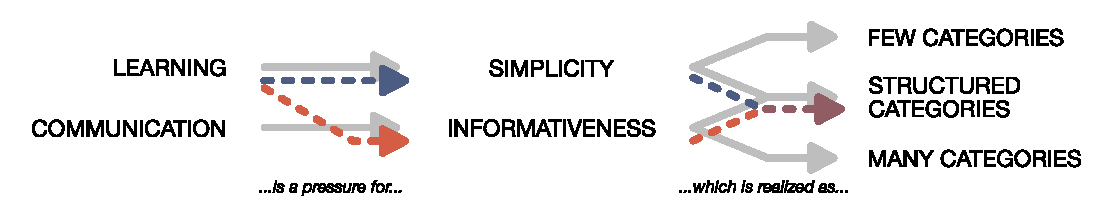
\includegraphics[]{fig15.eps}}
	\vspace*{2pt}
	\caption{Gray arrows show our general theoretical perspective: Pressure from learning alone favors simplicity which is realized as a small number of structured categories, while pressure from communication alone favors informativeness which is realized as a large number of structured categories. \textcite{Carstensen:2015} posit that learning might act as a pressure for informativeness, and this hypothesis is seemingly confirmed by the emergence of structured categories (red arrows). Our explanation says that this emergent structure is more likely to come directly from a pressure for simplicity (blue arrows).}
	\label{fig15}
	\end{figure}

Fig.~\ref{fig15} summarizes our argument. The gray arrows show our general theoretical perspective: Pressure from learning alone favors simplicity which is realized as a small number of structured categories, while pressure from communication alone favors informativeness which is realized as a large number of structured categories. In the two studies described by \textcite{Carstensen:2015}, there is, we contend, an increase in how structured the categories are over generational time,\footnote{Indeed, this is the only possible explanation for their finding that communicative cost decreases over generations. The systems start out with the maximum number of categories, which are approximately the same size, so the only possible way communicative cost can decrease is by restructuring the categories based on similarity.} a result that is consistent with the simplicity account (blue arrows) or the informativeness account (red arrows). However, Fig.~\ref{fig15} also highlights two important differences between the two accounts. First, the informativeness account requires positing a new learning bias in favor of informativeness, whereas the simplicity account is aligned with a large body of prior literature that links learning to simplicity \parencite[e.g.,][]{Solomonoff:1964a,Li:2008,Rissanen:1978,Chater:2003,Chater:2015,Culbertson:2016,Feldman:2016,Kemp:2012}. Second, although both accounts predict the emergence of structured categories, they diverge in terms of the number of categories that are expected to emerge: A bias for simplicity is expected to lead to the loss of categorical distinctions, while a bias for informativeness is expected to lead to an increase in the number of such distinctions. So this raises another question: If our simplicity account is correct, why did \textcite{Carstensen:2015} not observe a loss of categories?

In the case of Study~1 \parencite[i.e.,][]{Xu:2013}, participants were explicitly forced to use a certain number of categories according to condition, so there could be no category loss because of the particular design of the original study. In the case of Study~2, various explanations are possible, but we would suggest that the most likely explanation relates to the lack of a bottleneck on transmission. Participants were trained on all of the meanings, not a subset as is typical in iterated learning studies, so category loss is predicted to occur only very slowly. To illustrate this, we reran our model approximating the parameters of Study~2: Agents have an unweighted ($w=1$) simplicity prior and see all of the meanings ($b=4$, no bottleneck) in two exposures ($\xi=2$). The results are shown in Fig.~\ref{fig16} under three noise values. If we look only at the first 10 generations (left), there appears to be a small but sustained decrease in communicative cost, falling from 5~bits to around 4.7~bits,\footnote{Compare with \textcite[][Fig.~5]{Carstensen:2015}, where the decrease in communicative cost is similarly small, dropping from around 5.8~bits to 5.5~bits.} which suggests that the languages are becoming more informative. However, when the same model is observed over 100 generations (right), we find that the initial gain in informativeness is gradually eroded by the loss of categories. This is especially clear when the noise parameter is higher (e.g., $\epsilon=.1$), which causes category loss to happen faster.

	\begin{figure}
	\makebox[\textwidth][c]{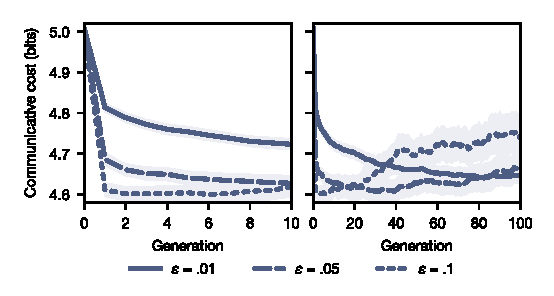
\includegraphics[]{fig16.eps}}
	\vspace*{2pt}
	\caption{Results for communicative cost under the simplicity prior for three settings of $\epsilon$. As in \textcite[][Study~2]{Carstensen:2015}, agents get two exposures ($\xi=2$) to all of the meanings ($b=4$). Over the course of 10 generations (left), the languages become more informative due to the structural simplification fostered by the simplicity prior. However, so long as $\epsilon > 0$, category loss---and therefore the erosion of this informativeness gain---is inevitable over a longer period of time (e.g., 100 generations; right). Increasing the noise level speeds the simplification process up.}
	\label{fig16}
	\end{figure}

When category loss is impeded, as is the case in the two studies reported by \textcite{Carstensen:2015}, the only way languages can simplify is by reorganizing how the categories are structured. Structure is achieved by grouping stimuli together based on similarity, and communicative cost measures this as an increase in informativeness. Crucially, we argue that this outcome---increased informativeness---is \textit{not} due to an inductive bias in favor of informativeness; it arises merely as a byproduct of increased simplicity.

The idea that compact structure is a form of simplicity has been argued in a number of places. For example, G{\"a}rdenfors's (\citeyear[p.~70]{Gardenfors:2000}) motivation for the naturalness of convexity (a correlate of compactness) is rooted in cognitive economy: ``I believe that [convexity] can be defended by a principle of \textit{cognitive economy}; handling convex sets puts less strain on learning, on your memory, and on your processing capacities than working with arbitrarily shaped regions.'' This view is supported by various studies showing how the application of a simplicity principle in learning favors a compact structural arrangement of concepts \parencite{Pothos:2009,SteinertThrelkeld:2019,Sims:2018}. Indeed, \textcite[p.~457]{Richie:2016} has also made this point in direct reference to \textcite{Carstensen:2015}, describing the authors' findings as a ``happy accident'' arising from the ``basic operation of categorization.''

It could, of course, be argued that humans have biases for both simplicity and informativeness. However, the point we wish to make in this paper is that a simplicity bias alone can already explain the decrease in communicative cost observed by \textcite{Carstensen:2015}, and since a domain-general bias for simplicity is very well motivated theoretically and empirically, this explanation should be preferred over positing an additional domain-specific bias for informativeness in language learning. This effectively means we are raising the bar on the evidence required to show that learning produces informative languages; evidence for this position must first rule out explanations from simplicity.

To complicate the issue further, there are at~least two ways compact structural arrangements could in principle emerge from \textit{communicative pressure} for informativeness, as we acknowledge in Fig.~\ref{fig15}. First, if the payoff from a communication game is not binary but related to the similarity between the speaker's intended meaning and the listener's inferred meaning \parencite[see e.g.,][]{Lantz:1964}, then interaction can provide pressure for compact structural representations. For example, \textcite{Jager:2007} have shown in agent-based simulations that compactly arranged color concepts can arise from a desire to minimize potential error in communication. Second, when faced with labeling a novel stimulus, speakers tend to assign the stimulus to an established category on the basis of similarity \parencite[e.g.,][]{Markman:1998} in order to maximize the probability of aligning with a listener, providing another route through which interaction can lead to compact structure. These lines of evidence have led \textcite{Warglien:2011} to promote a view in which both learning and communication contribute to structured categories.

The extent to which category structure derives from learning versus communication remains somewhat unclear. However, \textcite{Silvey:2019} have tackled precisely this issue by comparing results from (a) individual categorization, (b) communication games, (c) iterated learning, and (d) iterated learning with communication games. Among other things, the authors found that ``communication alone does not appear to be the best way to create category systems that are communicatively effective'' (p.~13); rather, the presence of (iterated) learning results in compactly structured categories that are effective for communication as a side-effect. They therefore argue that ``communication is neither necessary nor sufficient'' (p.~15) to explain the compact structure of semantic categories.

Finally, one potential criticism of this paper is that our stimuli are quite different from those used in \textcite{Carstensen:2015}, especially in terms of the integral--separable distinction. ``Integral dimensions are those that combine into relatively unanalyzable, integral wholes'' \parencite[p.~40]{Nosofsky:1986}; for example, when perceiving color, humans integrate information about hue, saturation, and brightness. In contrast, ``separable dimensions are highly analyzable and remain psychologically distinct when in combination'' \parencite[p.~40]{Nosofsky:1986}, the Shepard circles being classic examples of such stimuli, since the angle and size features can be perceived and categorized separately. Both of Carstensen et al.'s (\citeyear{Carstensen:2015}) studies use stimuli with integral dimensions (color and spatial relationships), which raises the possibility that our results might not offer a fair comparison to their work.

However, our choice of separable dimensions was, in~fact, a deliberate one. To see why, imagine we had designed our model and experiments around an integral space (e.g., color space). In such a space, the rectangle code would not be an appropriate measure of complexity; instead, a reasonable measure of complexity might be based around storing prototypes \parencite[see e.g.,][for an example of such an approach]{Pothos:2009}. When plugged into our model, this definition of simplicity would favor categories that have a compact, but multidimensional, structural organization. Such structure (which we just motivated by a preference for simplicity) would be indistinguishable from the structure predicted by the informativeness bias as formalized by communicative cost. Separable stimuli make it easier to distinguish between the predictions of an informativeness bias (maintenance of the four categories with a tendency toward the quadrant partition) versus the predictions of a simplicity bias (loss of categories with a tendency toward striped partitions).

%%%%%%%%%%%%%%%%%%%%%%%%%%%%%%%%%%%%%%%%%%%%%%%%%%%%%%%%%%%%%%%%%%%%%%%%%%%%%%%%%%%
\section{Conclusion}
%%%%%%%%%%%%%%%%%%%%%%%%%%%%%%%%%%%%%%%%%%%%%%%%%%%%%%%%%%%%%%%%%%%%%%%%%%%%%%%%%%%

There is a long tradition in the cognitive and language sciences of explaining the structural properties of language in terms of the simplicity--informativeness tradeoff. Broadly speaking, we view the pressure for simplicity as deriving from learning and the pressure for informativeness as deriving from communicative interaction. When languages are both learned and used, they find a balance between being sufficiently simple and sufficiently informative. However, at least two studies \parencite{Carstensen:2015,Fedzechkina:2012} have suggested that human learners might have an inductive bias not just for simplicity but also for informativeness, short-circuiting the need for interaction as a necessary condition in the emergence of informative languages. We formalized this hypothesis in terms of an iterated learning model with Bayesian category learners and tested it in an experimental analog of that model. This tight combination of model and experiment allowed us to fully explicate the two positions and test them objectively.

Our findings supported the status quo: The human inductive bias is better characterized by a preference for simplicity, not informativeness. Furthermore, we showed how the application of a simplicity principle in learning could explain the apparently contradictory results described by \textcite{Carstensen:2015}: Under a bias for simplicity, iterated learning gives rise to simple category systems that happen to have one of the hallmark features of an informative category system---a compact structural organization. Thus, although it is true that informativeness, when defined a particular way, can emerge through iterated learning, this does \textit{not} imply that learners have a domain-specific bias for informativeness. Given that the stated aim of \textcite[p.~303]{Carstensen:2015} was to ``establish what process gives rise to the diverse attested systems of informative categories,'' this is an important distinction to make.

Treating learning and communication separately allows us to elucidate the unique contribution that each pressure makes to the structure of language, this paper being primarily concerned with the contribution that learning makes. However, considering the two pressures together reveals the interesting ways in which learning and interaction can work together. \textcite[][p.~1228]{Frank:2009} argue that ``communicators choose what they want to say by how informative it would be about their intended meaning;'' thus, the data from which learners typically induce simple hypotheses is often explicitly designed, by the speaker, to be informative in a given context. This suggests an important role for pragmatics in shaping language; the true source of informativeness may lie in the production of data for an audience \parencite[as argued by][]{Kirby:2015} and in a given context \parencite[as argued by][]{Winters:2018}. In this sense, informativeness does ultimately derive from a cognitive source, but that source is pragmatic reasoning, not learning.

%%%%%%%%%%%%%%%%%%%%%%%%%%%%%%%%%%%%%%%%%%%%%%%%%%%%%%%%%%%%%%%%%%%%%%%%%%%%%%%%%%%
\section{Research Data}
%%%%%%%%%%%%%%%%%%%%%%%%%%%%%%%%%%%%%%%%%%%%%%%%%%%%%%%%%%%%%%%%%%%%%%%%%%%%%%%%%%%

The raw data and code that support both the model and the experiment are available from the public data archive associated with this project: https://osf.io/hkxqp

%%%%%%%%%%%%%%%%%%%%%%%%%%%%%%%%%%%%%%%%%%%%%%%%%%%%%%%%%%%%%%%%%%%%%%%%%%%%%%%%%%%
\section{Supplementary Material}
%%%%%%%%%%%%%%%%%%%%%%%%%%%%%%%%%%%%%%%%%%%%%%%%%%%%%%%%%%%%%%%%%%%%%%%%%%%%%%%%%%%

Model results under 48 parameter combinations: https://joncarr.net/p/shepard/

%%%%%%%%%%%%%%%%%%%%%%%%%%%%%%%%%%%%%%%%%%%%%%%%%%%%%%%%%%%%%%%%%%%%%%%%%%%%%%%%%%%
\section{Acknowledgments}
%%%%%%%%%%%%%%%%%%%%%%%%%%%%%%%%%%%%%%%%%%%%%%%%%%%%%%%%%%%%%%%%%%%%%%%%%%%%%%%%%%%

We thank Terry Regier and two other reviewers for their comments on previous versions of this paper. This work was supported by the Economic and Social Research Council (grant number ES/J500136/1).

\printbibliography

\end{document}